\begin{lemma}
    Consider the parabola defined as
    \begin{align}
        \label{quadform/app/1/quadratic}
        y &= ax^2+bx+c 
\\
  \text{or, }  \vec{x}^T\vec{V}\vec{x} + 2\vec{u}^T\vec{x} + f &= 0
\end{align}
%
where
\begin{align}
    \vec{V} &= \myvec{a & 0 \\ 0 & 0}
    \\
    \vec{u} &= \myvec{\frac{b}{2} \\ \frac{-1}{2}}
    \\
    f &= c
\\
        \eta &= \vec{u}^T\vec{p_1} = \frac{-1}{2}
    \end{align}
    

%
with  eigenvalue decomposition
\begin{align}
    \vec{D} &= \myvec{0 & 0 \\ 0 & a} \\
    \vec{P} &= \myvec{0 & 1 \\ 1 & 0}
\end{align}

Then the quadratic equation in         \eqref{quadform/app/1/quadratic} will not have real roots if 
\begin{align}
    \label{quadform/app/1/imag}
    \boxed{(\vec{p_1}^T\vec{c})(\vec{p_2}^T\vec{V}\vec{p_2}) > 0}
\end{align}
    
\end{lemma}
\begin{proof}
For the quadratic equation to not have any real roots, the y coordinate should always be either positive or negative . Express this in terms of the matrix/vector parameters of the parabola.  Now,for y coordinate to be always positive,two conditions need to be satisfied:
\begin{enumerate}
 \item y-coordinate of vertex $\vec{c}$ of parabola needs to be always positive.
 \item Coefficient $a$ of $x^2$ needs to be always positive.
\end{enumerate}
$\therefore$ For condition 1,
\begin{align}
    \myvec{\vec{u}^T + \eta\vec{p_1}^T \\ \vec{V}}\vec{c} &= \myvec{-f \\ \eta\vec{p_1}-\vec{u}} \\
    \vec{p_1}^T\vec{c} &> 0
\end{align}
and for condition 2,
\begin{align}
    \vec{p_2}^T\vec{V}\vec{p_2} > 0
\end{align}
Also, for y coordinate to be always negative, two conditions need to be satisfied:
\begin{enumerate}
 \item y-coordinate of vertex $\vec{c}$ of parabola needs to be always negative.
 \item Coefficient $a$ of $x^2$ needs to be always negative.
\end{enumerate}
$\therefore$ for condition 1,
\begin{align}
    \myvec{\vec{u}^T + \eta\vec{p_1}^T \\ -\vec{V}}\vec{c} &= \myvec{-f \\ \eta\vec{p_1}-\vec{u}} \\
    \vec{p_1}^T\vec{c} &< 0
\end{align}
and for condition 2,
\begin{align}
    \vec{p_2}^T\vec{V}\vec{p_2} < 0
\end{align}
All the above  can be clubbed together to obtain     \eqref{quadform/app/1/imag}.
\end{proof}
\subsection{Examples}
\begin{enumerate}
    \item 
    \begin{align}
        y &= 21x^2-28x+10
    \end{align}
    Here,
    \begin{align}
        \vec{V} = \myvec{21 & 0 \\ 0 & 0},\vec{u}=-\myvec{14 \\ \frac{1}{2}},f=10
    \end{align}
    Using eigenvalue decomposition,
    \begin{align}
        \vec{D} = \myvec{0 & 0\\0 & 21} ,\vec{P}=\myvec{0 & 1\\1 & 0}
    \end{align}
    $\therefore$Vertex $\vec{c}$ is given by
    \begin{align}
        \myvec{-14 & -1 \\ 21 & 0 \\ 0 & 0}\vec{c} &= \myvec{-10 \\ 14 \\ 0} \\
        \implies  \myvec{-14 & -1 \\ 21 & 0}\vec{c} &= \myvec{-10 \\ 14}
        \\
        \implies \vec{c} &= \myvec{\frac{2}{3} \\ \frac{2}{3}}
    \end{align}
    Now,
    \begin{align}
        \vec{p_1}^T\vec{c} &= \myvec{0 & 1}\myvec{\frac{2}{3} \\ \frac{2}{3}}
        \\
        &= \frac{2}{3}
    \end{align}
    and,
    \begin{align}
        \vec{p_2}^T\vec{V}\vec{p_2} &= \myvec{1 & 0}\myvec{21 & 0\\0& 0}\myvec{1 \\ 0}
        \\
        &= 21
    \end{align}
    $\because$
    \begin{align}
    (\vec{p_1}^T\vec{c})(\vec{p_2}^T\vec{V}\vec{p_2}) = (\frac{2}{3})(21) = \frac{42}{3}>0
    \end{align}
    Hence,the given equation does not have any real roots.
    
    \numberwithin{figure}{section}
    \begin{figure}[!ht]
    \centering
     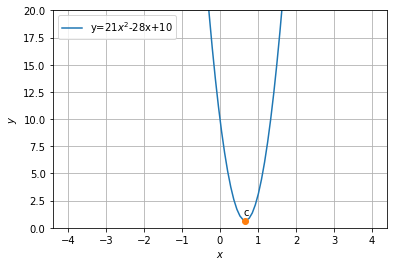
\includegraphics[width=\columnwidth]{app/1/Figures/ChallengeProblem3_2.png}
    \caption{$y=21x^2-28x+10$}
    \label{quadform/app/1/ex1}	
    \end{figure}
    
    \item
    \begin{align}
        y &= 6x^2-x-2
    \end{align}
    Here,
    \begin{align}
        \vec{V} = \myvec{6 & 0 \\ 0 & 0},\vec{u}=-\myvec{\frac{1}{2} \\ \frac{1}{2}},f=-2
    \end{align}
    Using eigenvalue decomposition,
    \begin{align}
        \vec{D} = \myvec{0 & 0\\0 & 6} ,\vec{P}=\myvec{0 & 1\\1 & 0}
    \end{align}
    $\therefore$Vertex $\vec{c}$ is given by
    \begin{align}
        \myvec{\frac{-1}{2} & -1 \\ 6 & 0 \\ 0 & 0}\vec{c} &= \myvec{2 \\ \frac{1}{2} \\ 0} \\
        \implies  \myvec{\frac{-1}{2} & -1 \\ 6 & 0}\vec{c} &= \myvec{2 \\ \frac{1}{2}}
        \\
        \implies \vec{c} &= \myvec{\frac{1}{12} \\ \frac{-49}{24}}
    \end{align}
    Now,
    \begin{align}
        \vec{p_1}^T\vec{c} &= \myvec{0 & 1}\myvec{\frac{1}{12} \\ \frac{-49}{24}}
        \\
        &= \frac{-49}{24}
    \end{align}
    and,
    \begin{align}
        \vec{p_2}^T\vec{V}\vec{p_2} &= \myvec{1 & 0}\myvec{6 & 0\\0& 0}\myvec{1 \\ 0}
        \\
        &= 6
    \end{align}
    $\because$
    \begin{align}
    (\vec{p_1}^T\vec{c})(\vec{p_2}^T\vec{V}\vec{p_2}) = (\frac{-49}{24})(6) = \frac{-49}{4}<0
    \end{align}
    Hence,the given equation has real roots.
    
    \numberwithin{figure}{section}
    \begin{figure}[!ht]
    \centering
     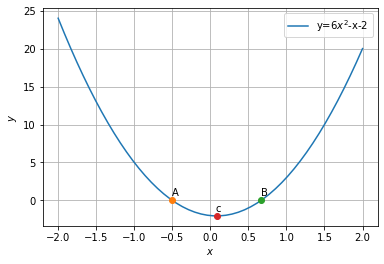
\includegraphics[width=\columnwidth]{app/1/Figures/ChallengeProblem3_1.png}
    \caption{$y=6x^2-x-2$}
    \label{quadform/app/1/ex2}	
    \end{figure}
    
    \item
    \begin{align}
        y &= -x^2-4x-5
    \end{align}
    Here,
    \begin{align}
        \vec{V} = \myvec{-1 & 0 \\ 0 & 0},\vec{u}=-\myvec{2 \\ \frac{1}{2}},f=-5
    \end{align}
    
    Using eigenvalue decomposition,
    \begin{align}
        \vec{D} = \myvec{0 & 0\\0 & -1} ,\vec{P}=\myvec{0 & 1\\1 & 0}
    \end{align}
    $\therefore$Vertex $\vec{c}$ is given by
    \begin{align}
        \myvec{-2 & -1 \\ 1 & 0 \\ 0 & 0}\vec{c} &= \myvec{5 \\ 2 \\ 0} \\
        \implies  \myvec{-2 & -1 \\ 1 & 0}\vec{c} &= \myvec{5 \\ 2}
        \\
        \implies \vec{c} &= \myvec{2\\-1}
    \end{align}
    
    Now,
    \begin{align}
        \vec{p_1}^T\vec{c} &= \myvec{0 & 1}\myvec{2 \\ -1}
        \\
        &= -1
    \end{align}
    and,
    \begin{align}
        \vec{p_2}^T\vec{V}\vec{p_2} &= \myvec{1 & 0}\myvec{-1 & 0\\0& 0}\myvec{1 \\ 0}
        \\
        &= -1
    \end{align}
    
    \numberwithin{figure}{section}
    \begin{figure}[!ht]
    \centering
     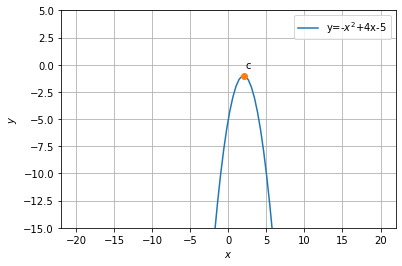
\includegraphics[width=\columnwidth]{app/1/Figures/ChallengeProblem3_3.png}
    \caption{$y=-x^2+4x-5$}
    \label{quadform/app/1/ex4}	
    \end{figure}
    
    $\because$
    \begin{align}
    (\vec{p_1}^T\vec{c})(\vec{p_2}^T\vec{V}\vec{p_2}) = (-1)(-1) = 1>0
    \end{align}
    Hence,the given equation does not have real roots.
  
    \item
    \begin{align}
        y &= -x^2-4x+9
    \end{align}
    Here,
    \begin{align}
        \vec{V} = \myvec{-1 & 0 \\ 0 & 0},\vec{u}=-\myvec{2 \\ \frac{1}{2}},f=9
    \end{align}
  
    Using eigenvalue decomposition,
    \begin{align}
        \vec{D} = \myvec{0 & 0\\0 & -1} ,\vec{P}=\myvec{0 & 1\\1 & 0}
    \end{align}
    $\therefore$Vertex $\vec{c}$ is given by
    \begin{align}
        \myvec{-2 & -1 \\ 1 & 0 \\ 0 & 0}\vec{c} &= \myvec{-9 \\ 2 \\ 0} \\
        \implies  \myvec{-2 & -1 \\ 1 & 0}\vec{c} &= \myvec{-9 \\ 2}
        \\
        \implies \vec{c} &= \myvec{2\\13}
    \end{align}
    
    \numberwithin{figure}{section}
    \begin{figure}[!ht]
    \centering
    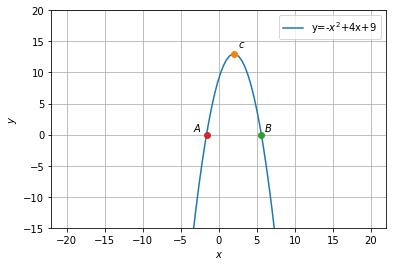
\includegraphics[width=\columnwidth]{app/1/Figures/ChallengeProblem3_4.png}
    \caption{$y=-x^2+4x+9$}
    \label{quadform/app/1/ex3}	
    \end{figure}
    
    Now,
    \begin{align}
        \vec{p_1}^T\vec{c} &= \myvec{0 & 1}\myvec{2 \\ 13}
        \\
        &= 13
    \end{align}
    and,
    \begin{align}
        \vec{p_2}^T\vec{V}\vec{p_2} &= \myvec{1 & 0}\myvec{-1 & 0\\0& 0}\myvec{1 \\ 0}
        \\
        &= -1
    \end{align}
    $\because$
    \begin{align}
    (\vec{p_1}^T\vec{c})(\vec{p_2}^T\vec{V}\vec{p_2}) = (13)(-1) = -13<0
    \end{align}
    Hence,the given equation has real roots.
\end{enumerate}

